
\chapter{Mathai-Quillen formula}
\label{chapter_mq}
The Mathai-Quillen formula is an explicit differential form representative of 
the Thom class of a vector bundle. The significance of the Thom class is 
that its pullback by a section to the base manifold gives a representative of the Euler
class, thus it can be used to calculate the Euler number of the vector bundle.  
Recall that there are two quite different approaches for calculating the Euler number
$\chi(X) = \chi(TX)$ of an oriented even dimensional manifold $X$. 
This first is topological, and counts
the signed isolated zeros of a vector field on $X$, via the Poincar\'e-Hopf theorem. The
second is differential geometric and represents  $\chi(X)$ as the integral over
$X$ of a density constructed from the curvature of a connection on $X$, via
the Gauss-Bonnet theorem. 
The Mathai-Quillen representative of the class depends on both a section $s$ and 
connection  $\nabla$ on the vector bundle, and can be regarded as a formula 
which interpolates between the two approaches.  

Our interest in the formula is further motivated by its application in providing a
geometric interpretation of the action principle of Witten's TQFT, where he
characterised Donaldson invariants as correlation functions of observables, as
we will see later in Chapter \ref{chapter_aj}. 

\section{Integration along the fiber} \label{section:fiber_integration}
Let $\pi: E\to B$ be an oriented fiber bundle over a manifold $B$ with oriented
fiber $F$. Suppose $\dim F = m$ and $\dim B = n$.
\begin{defn}
	\underline{Integration along the fiber} is a map $\pi_* : \Omega^*(E)\to
	\Omega^{*-m}(B)$, defined as follows. Let $\alpha\in \Omega^k(E)$ and
	$v_1,\ldots,v_{k-m} \in T_bB$, then $\pi_*$ is given by 
	\[
	(\pi_*\alpha)_b(v_1,\ldots,v_{k-m}) = \int_{\pi^{-1}(b)}
	\alpha(\widetilde{v}_1,\ldots,\widetilde{v}_{k-m},-)
	\] 
	where $\widetilde{v}_i$ is any lift of $v_i$ to $TE$. 
The integral is computed by pulling back the form via a trivialisation $\phi 
:F \xrightarrow{\simeq} \pi^{-1}(b)$. 
\end{defn}
\begin{figure}[htb]
	\hfill
	\begin{minipage}[c]{0.5\textwidth}
	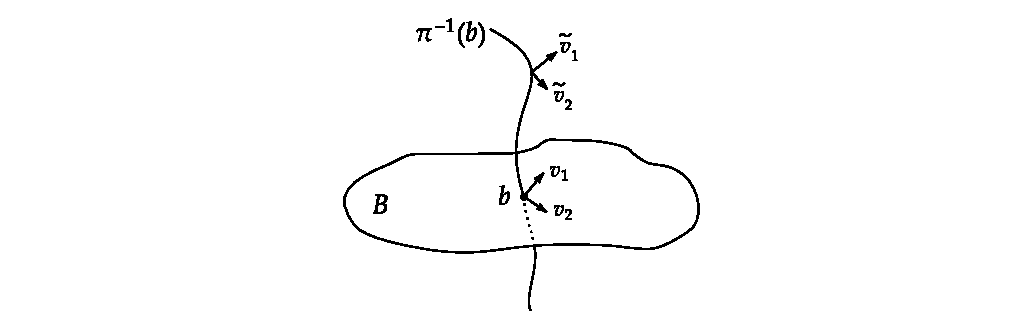
\includegraphics[trim={5cm 5mm 5cm 3mm},clip,width=\textwidth]{figs/fiber_integral.pdf}
	\end{minipage} 
	\begin{minipage}[c]{0.44\textwidth}
	\caption{Lift of tangent vectors along $\pi^{-1}(b)$}
	\label{fig:fiber_integral}
	\end{minipage} 
\end{figure}
To show that this is well defined, we need to check 
\begin{itemize}
	\item the integral is independent of choice of trivialisation
	\item definition is independent of the choices of lifts
	\item integrand is a smooth differential form on $\pi^{-1}(b)$
	\item $\pi_*\alpha$ is a smooth differential form on $B$
\end{itemize}
Denote $\beta = \alpha(\widetilde{v}_1,\ldots,\widetilde{v}_{k-m},-)$.\\
(1) Choice of trivialisation. This comes from the fact that the trivialisation
is oriented: if $\phi_1,\phi_2 : F \to \pi^{-1}(b)$ are two trivialisations,
then $\psi:=\phi_1^{-1}\phi_2 : F \to F$ is an orientation preserving diffeomorphism. 
Hence, on an open subset $V_\alpha \subset F$ the integral is written in
coordinates as  
\[
\int_{V_{\alpha}} \phi_1^*\beta \odif{f_1}\ldots\odif{f_m} 
= \int_{V_\alpha} \psi^*\phi_1^*\beta  \odif{g_1}\ldots\odif{g_m}
\] 
where $g_i = \psi(f_i)$ are the transformed coordinate functions. Since
$\det(D\psi)=1$ by assumption, the two integrals are equal by the change of 
coordinates theorem. 

Moreover, for vector bundles and principal bundles, the definition is also 
independent of the choice of oriented trivialisation with the same orientation. 
Even if $\phi_1,\phi_2$ are taken from different trivialisations, the
transition function $\phi_1^{-1}\phi_2: F \to F$ will be an orientation
preserving diffeomorphism due to the extra structure on $\phi_1$ and
$\phi_2$, i.e. linear isomorphism or $G$-equivariant map. 

(2) Choice of lifts. Fix $a\in \pi^{-1}(b)$, and let $\widetilde{v}_1'$ be 
another lift of $v_1\in T_bB$. That is, 
$D\pi|_a(\widetilde{v}_1)=D\pi|_a(\widetilde{v}_1')=v_1$. So
$\widetilde{v}_1'-\widetilde{v}_1\in \ker D\pi|_a = T_a(p^{-1}(b))$.  

Since the fiber dimension is $m$, $m+1$ vectors 
$w_1,\ldots,w_m,\widetilde{v}_1'-\widetilde{v}_1 \in T_a(\pi^{-1}(b))$ are
linearly dependent, and therefore 
\[
\alpha(\widetilde{v}_1'-\widetilde{v}_1,
\widetilde{v}_2,\ldots,\widetilde{v}_{k-m},w_1,\ldots,w_m) = 0
\] 
which shows the integrand is independent of the choice of lifts.

(3) Integrand is smooth on $\pi^{-1}(b)$. Since $\alpha$ is a smooth 
differential form, we only need to check that its dependence on the lifted 
vectors is smooth. Given a local trivialisation $\phi : U\times F
\xrightarrow{\simeq} \pi^{-1}(U)$, at $a\in\pi^{-1}(b)$ we can choose the lift 
$\widetilde{v}_1 = D\phi|_{\phi^{-1}(a)}(v_1)$. This is a smooth choice, and
hence $\alpha$ is smooth by part (2). 

(4) $\pi_*\alpha$ is a smooth differential form on $B$. To see this, we can
write it out in coordinates. Let 
$dx_1,\ldots,dx_{n},dt_1,\ldots,dt_m \in T^*E|_U$ be a basis, where
$t_i$ are coordinate functions for $F$ and $x_i$ are coordinate functions for
$B$. Assume $\alpha$ is a product of 1-forms and has a factor of 
$dt_1\wedge \cdots\wedge dt_m$, since
otherwise $\beta$ will not be a top form on $\pi^{-1}(b)$. Then integration
along the fiber is locally described by 
\[
\alpha = \pi^*\eta \wedge f(x,t) \odif{t_1}\cdots \odif{t_m}   
\mapsto \eta\wedge \int_{\pi^{-1}(b)} f(x,t) \odif{t_1}\cdots \odif{t_m}
\] 
for some $\eta\in \Omega(B)$. It is now apparent that the dependence on $x$,
i.e. the coordinates for  $B$, is smooth. 
\begin{remark}
	Note that not all differential forms in $\Omega^*(E)$ are integrable, 
	so we typically restrict the domain of $\pi_*$ to some space of integrable
	forms. For now, assume this has been done.
\end{remark}
In this chapter, we are interested in integration along the fiber for oriented
vector bundles in particular, however the general definition will be needed
later when we integrate over $G$-orbits of principal bundles. The case of vector
bundles is slightly simpler, because the fiber has global coordinates. 
\begin{prop} % Bott Tu p62
	Integration along the fiber $\pi_*$ commutes with the exterior derivative
	$d$.
\end{prop}
\begin{proof}
	Since $\pi_*$ and  $d$ are linear,
	it suffices to prove this proposition on the restriction $E|_U \simeq
	U\times F$ to a subset in the trivialising open cover. If $\omega\in
	\Omega^*(E)$, to write it in coordinates we need to further choose a
	subset $U\times V$ which is diffeomorphic to an open neighbourhood of
	$\mathbb{R}^{n+m}$. Then
	we can write it locally as $\omega = \pi^*\eta \wedge f(x,t) dt_1\cdots
	dt_n$ for some $\eta\in \Omega^*(B)$. Then 
	\begin{align*}
		d\pi_*\omega
		&= d \paren{\eta\wedge \int f(x,t)\odif{t_1}\cdots\odif{t_m} } \\
		&= d\eta\wedge\int f(x,t)\odif{t_1}\cdots\odif{t_m}  
		+\eta\wedge \sum_i dx_i\int \partial_{x_i} f(x,t)\odif{t_1}\cdots\odif{t_m} 
	\end{align*}
	and 
	\begin{align*}
		\pi_*d\omega
		&= \pi_*\paren[2]{\pi^*d\eta\wedge f(x,t) dt_1\cdots
		dt_n + \pi^*\eta \wedge\sum_i \partial_{x_i}f(x,t) dx_i dt_1\cdots
		dt_n } \\
		&= d\eta\wedge\int f(x,t)\odif{t_1}\cdots\odif{t_m} + \eta \wedge
		\sum_i dx_i\int \partial_{x_i} f(x,t)\odif{t_1}\cdots\odif{t_m} 
	\end{align*}
	where we have used $d\pi^*\eta = \pi^*d\eta$ in the first line. The proof is
	concluded by summing over the partition of unities subordinate to
	trivialising covers of $F$ and $E$.
\end{proof}
Therefore, $\pi_*$ descends to a well defined map on de Rham cohomology. 
Integration along the fiber can also be defined by the property (b) in the
following proposition, where the existence of $\pi_*\alpha$ can be seen as a 
generalisation of Fubini's theorem.
Here $\Omega_c^*(E)$ denotes the space of forms with compact support, while 
$\Omega_{cv}^*(E)$ denotes the space of forms with compact support along the
fiber: $\omega$ is in $\Omega_{cv}^*(E)$ if for every compact set $K \subset B$, 
$\pi^{-1}(K)\cap \supp(\omega)$ is compact in $E$. 
\begin{prop}[Projection formula] %  Bott Tu Prop 6.15 p63, BGV 1.15
	\label{prop:projection_formula}
	Let $\pi : E \to B$ be a fiber bundle with  $m$-dimensional fiber $F$, and
	both $B$ and  $E$ are oriented. 
	\begin{enumerate}[(a), leftmargin=\parindent]
	    \item For $\alpha\in \Omega_{cv}(E)$ and $\beta\in\Omega(B)$, 
	\[
		\beta\wedge \pi_*\alpha = \pi_*(\pi^*\beta\wedge\alpha)  
	\] 
		\item If $\alpha \in \Omega_{cv}(E)$ and $\beta\in \Omega_{c}(B)$,
			\[
			\int_B \beta\wedge \pi_*\alpha =  \int_E \pi^*\beta\wedge\alpha
			\] 
	\end{enumerate}
\end{prop}
\begin{proof}
	(a) Write $\alpha = \pi^*\eta \wedge f(x,t) dt_1\wedge\cdots\wedge dt_m $
	in terms of local coordinates on $E|_U$. Then 
	\[
	\pi_*(\pi^*\beta\wedge \alpha)
	=\pi^*(\beta\wedge\eta)\wedge \int_{\pi^{-1}(b)}f(x,t) 
	dt_1\wedge\cdots\wedge dt_m 	
	= \beta\wedge\pi_*(\alpha)
	\] 
	Note that there is an implicit sum over a partition of unity for $F$.\\
	(b) Again, it suffices to prove this on the restriction $E|_U\simeq U\times F$ to a
	subset in the trivialising cover for $E$. Furthermore,
	let $U\times V_\alpha$ be a trivialising open cover of $U\times F$, 
	where $U$ and each $V_{\alpha}\subset F$ are diffeomorphic to an open subset of
	$\mathbb{R}^d$. After summing over the partition of unity
	subordinate to an open cover of $E$, 
	the result will still hold. On $E|_U$, the integral can be written
	\begin{align*}
		\int_{E|_U} \pi^*\beta\wedge \alpha
		&= \sum_\alpha\int_{U \times V_\alpha}\pi^*\beta\wedge \alpha \\
		&= \sum_\alpha\int_{U}\int_{V_\alpha}\pi^*\beta\wedge \alpha
		= \int_{U}\int_{\pi^{-1}(b)}\pi^*\beta\wedge \alpha
		= \int_{U}\beta\wedge \pi_*\alpha 
	\end{align*}
	where we have applied Fubini's theorem in the second line, and the result of
	part (a) in the last equality.
\end{proof}


\section{Thom isomorphism}
\begin{thm}[Poincar\'e duality {\cite[p.44]{bott_tu}}] 
	\label{thm:poincare_duality}
	If $M$ is an oriented manifold of dimension $n$, then the pairing 
	\[
	\int_M : H^q(M)\otimes H_c^{n-q}(M) \to \mathbb{R}
	\] 
	is non-degenerate. Therefore, $H^q(M)\simeq (H^{n-q}_c(M))^*$. 
\end{thm}

Consider a vector bundle $E\to M$ of rank  $n$, over a manifold of dimension $m$. 
Since the zero section embeds
$M$ in  $E$, $M$ is a deformation retract of  $E$. Since
homotopic maps induce the same map in de Rham cohomology, it follows that
\[
H^*(E) \simeq H^*(M)
\] 
If we further assume $E$ and  $M$ are orientable manifolds, 
then a similar statement also holds for compact cohomology using 
Poincar\'e duality % Bott Tu pg 60
\[
H^*_c(E) \simeq (H^{n+m-*}(E))^* \simeq (H^{n+m-*}(M))^* \simeq H^{*-n}_c(M)
\] 
The Thom isomorphism is concerned with compact vertical cohomology. 
From the previous section, integration along the fiber descends to a map 
on compact vertical cohomology
$\pi_* : H_{cv}^*(E) \to H^*(M)$. In fact, we can show that it induces an
isomorphism, called the Thom isomorphism.
We shall prove this in the trivial bundle case $M\times \mathbb{R}^n \to M$.
\begin{prop} % Bott Tu Prop 6.16 
	Integration along the fiber defines an isomorphism
	\[
	\pi_* : H_{cv}^*(M\times \mathbb{R}^n) \to H^{*-n}(M)
	\] 
\end{prop}
\begin{proof} % p38 
	Let $\pi^n_* : H_{cv}^*(M\times \mathbb{R}^n) \to H_{cv}^{*-1}(M\times
	\mathbb{R}^{n-1})$ be integration along the last component of
	$\mathbb{R}^n$, and for ease of notation denote $H_{cv}^*(M\times
	\mathbb{R}^0) := H^*(M)$. We will prove that $\pi^n_*$ defines an
	isomorphism, because then the proposition follows by taking the composition
	$\pi_* = \pi^1_* \circ \cdots\circ \pi^n_*$ (using Fubini's theorem).

	Let $dt:=dt_1\wedge \cdots\wedge dt_n\in\Omega^n(\mathbb{R}^n)$ be the top 
	form corresponding to orthonormal coordinates on $\mathbb{R}^n$. 
	To produce a map in the reverse direction to $\pi^n_*$, let $e(t)dt \in
	\Omega^1_c(\mathbb{R})$ be a compactly supported $1$-form with integral 1,
	and define 
	\begin{align*}
	e_* : \Omega_{cv}^*(M\times \mathbb{R}^{n-1}) \to 
	\Omega^{*+1}_{cv}(M\times \mathbb{R}^n), \qquad  
	\omega \mapsto \omega \wedge e(t_n)\, dt_n 
	\end{align*}
	It is clear that $e_*$ commutes with  $d$, so induces a map on cohomology.
	Moreover,  $\pi_*^n \circ e_* = 1$ on  $\Omega_{cv}^*(M\times
	\mathbb{R}^{n-1})$. While $e_*\circ
	\pi_*^n \neq 1$ on the levels of forms, our strategy is to construct a
	homotopy operator  $K:\Omega^{*}(M\times \mathbb{R}^n) \to
	\Omega^{*-1}(M\times \mathbb{R}^n)$ such that 
	\begin{equation} \label{eq:homotopy_operator}
		1-e_*\pi_*^n = (-1)^{q-1}(dK-Kd), \qquad 
		\text{on } \Omega^q(M\times \mathbb{R}^n)
	\end{equation}
	This will imply that for any closed $\omega \in \Omega^*(M\times
	\mathbb{R}^n)$, $(1-e_*\pi_*^n)\omega$ is proportional to  $dK\omega$, 
	which is exact. Thus $e_*\pi_*^n=1$ on cohomology.
	Let $\omega \in \Omega^*(M\times \mathbb{R}^n)$. If $\omega$ does not 
	contain a factor of  $dt_n$, define $K(\omega) = 0$. Otherwise define 
	\[
		\omega = (\pi^*\phi) f(x,t) dt_I dt_n \mapsto 
		\pi^*\phi dt_I\paren[2]{\int_{-\infty}^t f \odif{t_n} 
		- \int_{-\infty}^t e \odif{t_n} \int_{\mathbb{R}} f \odif{t_n}}
	\] 
	where $I \subset \{1,\ldots,n-1\}$.
	It is now straightforward to prove equation (\ref{eq:homotopy_operator}):
	compute and compare $(dK-Kd)\omega$ with $(1-e_*\pi_*^n)\omega$ for the cases 
	where $\omega$ contains a factor of $dt_n$ or not.
\end{proof}
The proof above shows that the inverse map in cohomology is given by the wedge
product with a compactly supported form $\Phi \in \Omega^{n}(\mathbb{R}^n)$ 
whose integral along each component is 1. This can be generalised to arbitrary 
vector bundles $E\to M$, known as the Thom isomorphism. 

\begin{thm}[Thom Isomorphism {\cite[Theorem 6.17]{bott_tu}}] % Thm 6.17 Bott Tu
	For a vector bundle $E$ over compact manifold $M$,
	integration along the fiber induces an isomorphism
	 $H^*_{cv}(E) \simeq H^{*-n}(M)$
\end{thm}
\begin{defn}
	Under the Thom isomorphism $H^*(M)\to H_{cv}^{*+n}(E)$, the
	image of $1\in H^0(M)$ is called the \underline{Thom class}  $\Phi\in
	H_{cv}^n(E)$ of the vector bundle.
\end{defn}
In other words, the representatives of the Thom class are precisely the forms
which are compactly supported along the fiber and have integral 1 along the
fibers. As a direct consequence of Proposition \ref{prop:projection_formula},
the Thom class $\Phi \in H_{cv}^n(E)$ satisfies for all $\beta \in \Omega^*_c(M)$
\begin{equation} \label{eq:thom_form_property}
	\int_M \beta = \int_E \pi^*\beta \wedge \Phi
\end{equation}

% compact implies finite good cover = finite type 
% TODO generalise to non compact manifolds?

\section{Mathai-Quillen construction of Thom form}
\label{section:mq_formula}
The Mathai-Quillen construction uses a slight variation of the Thom isomorphism.
Differential forms with compact support in each fibre are replaced by forms
which are rapidly decreasing in the fibre directions. 

\begin{defn}
	Let $E\to M$ be a vector bundle with fiber  $V$ of rank  $n$.
	A differential form $\omega\in \Omega(E)$ is \underline{rapidly decreasing
	along the fiber} if the restriction to the fiber 
	$\omega_{\pi^{-1}(x)} : V \to \mathbb{R}$ is a Schwartz function for all $x\in M$,
	i.e.
	 \[
		 \fall a,b \in \mathbb{N}^n, \norm[*]{\omega_{\pi^{-1}(x)}}_{a,b} < \infty
	\] 
	where $\displaystyle \norm{f}_{a,b} := \sup_{x\in \mathbb{R}^n}\abs[*]{x^a(D^bf)(x)}$.
	The space of such forms is denoted $\Omega_{rd}(E)$.
\end{defn}

\vspace{-1ex}

\hspace{-7mm}
\begin{minipage}{0.5\textwidth}
Using the diffeomorphism $h : E \to E$ mapping the unit ball to $\mathbb{R}^n$
	\[
	h(y) = \frac{y}{\sqrt{1-\norm{y^2}} }
	\] 
\end{minipage}
\begin{minipage}{0.5\textwidth}
		\centering
		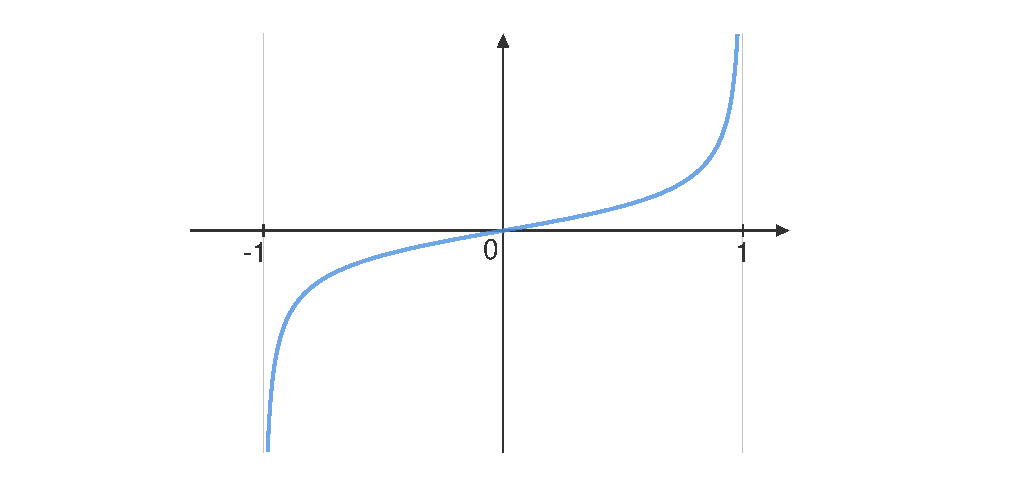
\includegraphics[trim={3cm 0 3cm 0},clip,width=\textwidth]{figs/rd_diffeomorphism.pdf}
\end{minipage}
we can pull back a rapidly decreasing form $\omega\in \Omega_{rd}^*(E)$ to 
$\Omega_{cv}^*(E)$ which is supported on the unit ball bundle. 
Note that the Schwartz property guarantees that $h^*\omega$ is smooth, i.e. 
all derivatives approach zero as $y \to 1$ since $\omega$ decays faster than any
polynomial.


Let us first look at the construction on an oriented Euclidean vector bundle
$E\xrightarrow{\pi} M$ of rank $n$ over a point $M=\{x_0\}$. 
Given coordinates $x^1,\ldots,x^n$ on $E$ from the local trivialisation,
a Thom form $U\in \Omega^n_{rd}(E)$ can be defined as
\[
	U(x) = (2\pi)^{-n/2}e^{-\abs{x}^2 /2} dx^1\wedge \ldots\wedge dx^n
\] 
Given the basis $e_1,\ldots,e_n$ of  $V$ corresponding to the coordinates
$x^1,\ldots,x^n$, denote the map $dx = dx^k \otimes e_k \in 
\Omega^1(E, V)$. Then $e^{-idx}\in \Omega(E,\bigwedge V)$ by taking a formal sum
of wedge products.
We can express this form in terms of the Berezin integral,
considered as a map $\int^B := \int \odif{e_1}\cdots\odif{e_n} 
: \Omega^*(E,\bigwedge V) \to \Omega^*(E)$. The reader is advised at this stage
to refer to Appendix \ref{appendix2} for the definition and properties of the 
Berezin integral, which will be utilised extensively in this chapter. 

\begin{lem} \label{lem:gaussian_integral} %1.49 BGV
	The form $U\in \Omega^n_{cv}(E)$ equals 
	\[
		 U(x) = (2\pi)^{-n/2} e^{-\abs{x}^2 /2} \epsilon(n)\int^B e^{-idx}
	\] 
	where $\epsilon(n)=1$ if  $n$ is even, otherwise  $i$.
\end{lem}
\begin{proof}
	The Berezin integral kills any forms of order less than $n$, so only
	multiples of $e_1 \wedge \ldots\wedge e_n$ remain.
	Hence,
	\begin{align*}
		\int^B e^{-idx} 
		&= (-i)^n \frac{1}{n!}\int^B (dx^k\otimes e_k)^n \\
		&= (-i)^n \int^B (dx^1\otimes e_1) \ldots(dx^n\otimes e_n) \\
		&= (-i)^n(-1)^{n(n-1)/2} \int^B dx^1\wedge \ldots\wedge dx^n\otimes e_1 \wedge\ldots\wedge e_n \\
		&= (-i)^n(-1)^{n(n-1)/2} dx^1\wedge \ldots\wedge dx^n
	\end{align*}
	Multiplication of elements of $\Omega(E,\bigwedge V)$ occur in
	the graded tensor product, so that this is a graded algebra. 
	In the second line, we have permuted all $n!$ terms into standard order, and
	terms of degree two commute.
	In the third line, $dx^i$ are separated from the  $e_i$, which
	anti-commute due to  $\Omega(E,\bigwedge V)$ being a graded algebra. 
	The lemma now follows, since
	$(-i)^n(-1)^{n(n-1)/2}$ equals 1 if $n$ is even, and otherwise  $-i$. 
\end{proof}
Our goal is to now define the Thom form on a more general manifold by 
modification of the above lemma. We define the   
\underline{tautological section} $x \in \Omega^0(E,\pi^*E)$ 
by $e\in E_p \mapsto e\in (\pi^*E)_{e} = E_{p}$.
Then choosing a Euclidean connection $\nabla^E$ on  $E$, we have an induced
covariant derivative $\nabla^{\pi^* E}$ on $\pi^* E \to E$, which we denote by
just $\nabla$.
Our idea is to replace  $dx$ by $\nabla^{\pi^*E} x \in \Omega^1(E,\pi^*E)$. 
In the rest of this section, denote $V=\pi^*E$ to simplify notation.

Next, recall that the curvature is a form in $\Omega^2(E,\End(V))$ 
which is skew-symmetric valued. We can identify $\mathfrak{so}(V)$ with 
$\bigwedge^2 V$ in the following way:
\begin{equation} \label{eq:so_wedge}
	A\in \mathfrak{so}(V) \mapsto \sum_{i<j} \gen{Ae_i,e_j} e_i\wedge e_j
\end{equation}
given a frame of $V$. Hence, we denote the curvature form as $F \in
\Omega^2(E,\bigwedge^2V)$.

We now define the Mathai-Quillen Thom form (corresponding to $t=1$)
\begin{equation}
	U_t = (2\pi)^{-n/2}\epsilon(n) \int^B e^{-\frac{1}{2}t^2\abs{x}^2-it\nabla x - F} \in \Omega^n(E)
\end{equation}
To justify why $U_t\in\Omega^n(E)$, note that
$\omega_t\in\bigoplus_{i=0}^2 \Omega^i(E,\bigwedge^iV)$, and hence 
$e^{-\omega_t} \in \bigoplus_{i=0}^n \Omega^i(E,\bigwedge^iV)$. The Berezin
integral then only retains the top degree part. 

To prove that $U$ is indeed a Thom form, we first need
to define a contraction operator $\iota(s):\Omega^i(E,\bigwedge^j V) \to
\Omega^i(E,\bigwedge^{j-1} V)$ for $s\in\Gamma(V)$ in
a similar fashion to definition \ref{def:contraction}, by the following
properties:
\begin{enumerate}[(1)]
    \item If $w\in \Omega^0(E,V)$, then  $\iota(s)w = \gen{s,w}$
	\item If $\alpha\in\Omega^i(E,\bigwedge^jV),
		\beta\in\Omega^k(E,\bigwedge^lV)$, then 
	 \[
	\iota(x)(\alpha\wedge \beta) 
	= (\iota(x)\alpha)\wedge\beta + (-1)^{i+j}\alpha\wedge(\iota(x)\beta)
	\] 
\end{enumerate}
Note that this uniquely defines $\iota(s)$ because the formulas can be applied
to a basis of the graded tensor product $\bigwedge^iT^*E\otimes \bigwedge^jV$.

\begin{prop} \label{prop:derivative_berezin} %1.50 BGV
	If $\nabla$ is a metric connection on  $\pi^*E$, this induces a covariant
	derivative on $\bigwedge \pi^*E$. Then for any
	$\alpha\in\Omega(E,\bigwedge V)$ and $s\in \Gamma(E,V)$, we have 
	\[
	d\int^B \alpha = \int^B \nabla\alpha = \int^B (\nabla-it\iota(s))\alpha
	\] 
\end{prop}
\begin{proof} 
	Given a non-vanishing section $\nu\in \Omega^1(E,\bigwedge^nV)$,
	the Berezin integral is given by the induced metric on $\bigwedge V$
	with  $\nu$. From section \ref{section:berezin_forms}, the induced covariant
	derivative $\nabla$ on $\bigwedge V$ is compatible with this metric, and 
	\[
	d\int^B\omega = d\gen{\nu,\omega} = \gen{\nabla \nu, \omega} + \gen{\nu, \nabla \omega}
	=\int^B \nabla\omega
	\] 
	where we have used the fact that $\nabla \nu = 0$, by definition of the
	Berezin integral on an oriented vector bundle with a metric connection.
	We can extend this to 
	$d\int^B\alpha = \int^B (\nabla-it\iota(s))\alpha$ for any section of
	$\pi^*E$ because $\iota(s)\alpha$ has no component in 
	the top exterior power.	
\end{proof}

\begin{prop} \label{prop:closed_prop} % 1.51 BGV
	Let $x \in \Gamma(E,V)$ be the tautological section on $E$, and $\nabla$ the
	induced connection on $\bigwedge V$.
	Let $\omega_t = \frac{1}{2}t^2\abs{x}^2 + it\nabla x + F 
	\in \Omega(E,\bigwedge V)$. Then 
	\[
		(\nabla - it\iota(x))\omega_t = 0
	\] 
\end{prop}
\begin{proof}
	 By metric compatibility,
	$\nabla \abs{x}^2 = 2\gen{\nabla x, x} = -2\iota(x)\nabla x$.
	Next, we have $\nabla(\nabla x) = \iota(x) F$.
	Finally by Bianchi's identity, $\nabla F = 0$. Combining this,
	\[
	\nabla \omega_t = -t^2\iota(x) \nabla x + it\iota(x)F 
	\] 
	On the other hand, $\iota(x)\abs{x}^2 = 0$ by definition of $\iota(x)$, so
	\[
	it\iota(x)\omega_t = -t^2\iota(x) \nabla x + it\iota(x)F
	\] 
	from which it follows that $(\nabla - it\iota(x))\omega_t = 0$.
\end{proof}

\begin{thm}
	The Mathai-Quillen form $U \in \Omega^n_{rd}(E)$ is a Thom form. 
\end{thm}
\begin{proof}
	% BGV Lemma 1.51
	We need to show that $U$ is closed, and integration along the fiber gives $1\in
	\Omega^0(E)$.
	From equation (\ref{eq:grassman_exp}), the exponential of $-\omega_t$
	can be written 
	\begin{equation} \label{eq:MQ_exp}
		e^{-\omega_t} = \sum_{k=0}^{n} \frac{e^{-t^2\abs{x}^2 /2}}{k!} (-it\nabla x
		- F)^k 
		= \sum_{k=0}^{\infty} \frac{1}{k!} (-\omega_t)^k
	\end{equation}
	Since $\nabla - it\iota(x)$ is an antiderivation, it follows from
	Proposition \ref{prop:closed_prop} that $(\nabla-it\iota(x)) e^{-\omega_t} =
	0$. 
	And therefore by Proposition \ref{prop:derivative_berezin}
	it follows that $U_t \propto \int^B e^{-\omega_t}$ is closed.
	
	% BGV prop 1.52 says integral reduces to the case where $M$ is a point
	% Proof is found from Blau 
	From equation (\ref{eq:MQ_exp}), we can write the Thom form as 
	\[
	U_t = (2\pi)^{-n/2}\epsilon(N) e^{-\frac{1}{2}\abs{x}^2}\int^B e^{-i\nabla x -F}
	\] 
	To integrate $U_t \in \Omega(E)$ along the fiber of $V=\pi^*E$, we extract from
	the Berezin integral the part which is a $n$-form on the fiber of $V$,
	\begin{align*}
		\int_E (2\pi)^{-n/2}\epsilon(n) e^{-\frac{1}{2}\abs{x}^2}\int^B e^{-i\nabla x -F}
		&= (2\pi)^{-n/2}\epsilon(n) \int_E e^{-\frac{1}{2}\abs{x}^2}\int^B 
		e^{-idx}
		= 1 
	\end{align*}
	we are only left with the $dx$ term because the induced connection and
	curvature forms on  $\pi^*E$ do not have any components along the fiber.
	We have evaluated the integral using Lemma \ref{lem:gaussian_integral}.
\end{proof}

%%%%%%%%%%%%%%%%%%%%%%%%%%%%%%%
\begin{comment} % Blau approach
Let $E=P\times_\rho V$ be the associated bundle to $P$ with rank $2m$. 
basic forms on $P\times V$ are in correspondence with forms on  $E$.

A representative for the Thom class, called the Mathai-Quillen Thom form, is
given by
\begin{equation} \label{eq:mathai_quillen}
\Phi_\nabla(E) = \frac{1}{(2\pi)^m} e^{-v_a^2/2} \int \odif{\chi} 
\exp(\chi_a\Omega^{ab}\chi_b /2 + i\nabla v^a \chi_a)
\end{equation}
where $v^a \in \Omega^0(P\times V)$ are coordinates on $V$, and $\nabla v^a \in
\Omega^1(P\times V)$ is the exterior covariant derivative of $v^a$.
Not well defined globally, since using trivialisation to use coordinates? 

We claim that this defines a basic form in $\Omega^{2m}_\rho(P\times V)$,
and that it is a representative of the Thom class. 

To show that it is a basic form, we need to prove it is horizontal and $\rho$
equivariant.  

To show that is is a representative of the Thom class, we need to prove it is
closed and satisfies  $\pi^*\Phi_\nabla(E) = 1$.

Pullback by zero section is Pfaffian.
\end{comment} 
%%%%%%%%%%%%%%%%%%%%%%%%%%%%%%%

Next, we will show one of the key properties of the Thom form: its pullback to
$M$ by any section  $s:M\to E$ is a representative of the Euler class of the
vector bundle. The Mathai-Quillen formula gives us a direct way to prove this, 
via the following transgression formula, which is the reason we defined the 
parameter $t$. 
\begin{lem} % prop 1.53 BGV
	The form $U_t \in \Omega^n(E)$ satisfies the transgression formula
	\[
	\odv{}{t} U_t = -i(2\pi)^{-n /2}\epsilon(n) d\int^B x e^{-\omega_t}
	\] 
\end{lem}
\begin{proof}
	With $\omega_t = \frac{1}{2}t^2\abs{x}^2+it\nabla x + F \in
	\Omega(E,\bigwedge V)$ as before, we have 
	\[
		\odv{\omega_t}{t} = t\abs{x}^2 + i\nabla x = i(\nabla - it\iota(x)) x
	\] 
	Since $(\nabla - it\iota(x))\omega_t = 0$ by Proposition
	\ref{prop:closed_prop}, we have 
	 \[
	\odv{}{t}e^{-\omega_t} = - \odv{\omega_t}{t} e^{-\omega_t} 
	= -i((\nabla	-it\iota(x))x) e^{-\omega_t}
	= -i(\nabla	-it\iota(x))(x e^{-\omega_t})
	\] 
	and hence by application of Proposition \ref{prop:derivative_berezin},
	\begin{align*}
		\odv{U_t}{t} 
		&= -i(2\pi)^{-n /2}\epsilon(n) \int^B (\nabla-it\iota(x))(x e^{-\omega_t})\\
		&= -i(2\pi)^{-n /2}\epsilon(n) d\int^B x e^{-\omega_t} 
	\end{align*}
\end{proof}
\begin{prop} \label{prop:thom_pullback}
	Let $s\in \Gamma(M,E)$ be a section of $E$.
	The cohomology class of the pullback $s^*U \in \Omega^{n}(M)$
	is independent of the section  $s\in\Gamma(E)$, and is a representative of
	the Euler class for even $n$.
\end{prop}
\begin{proof}
	First observe that $s^*U_0 = (2\pi)^{-n /2}\epsilon(n)\int^B e^{-s^*F} \in \Omega(M)$. 
	From equation (\ref{eq:so_wedge}), $F\in \Omega^2(E,\bigwedge^2 V)$ is 
	given in a frame of $V$ by
	 \[
	F = \sum_{i< j} F_{ji} e_i \wedge e_j
	= -\frac{1}{2}\sum_{i,j} F_{ij} e_i \wedge e_j
	\] 
	Since $F= \pi^* \Omega$ is the pullback of the curvature $\Omega$ on $E\to M$, the
	pullback of $F$ by any section $s$ gives the original curvature form, since
	$s^*\pi^* = (\pi\circ s)^*$. Therefore, $s^*U_0$ does not depend on $s$, and
	is equal to  $s^*U_0 = (2\pi)^{-n /2}\epsilon(n) \Pf(\Omega)$ by 
	Lemma \ref{lem:berezin_pf}, which is a representative of the Euler class
	from standard Chern-Weil theory. 

	To show this also holds for $s^*U$, 
	we can integrate the transgression formula above from 0 to 1, 
	\[
		U_1 - U_0 = -i(2\pi)^{-n /2}\epsilon(n)d\int_0^1\int^B x e^{-t^2\abs{x}^2/2 -
		it\nabla x - F} \odif{t}
	\] 
	Then taking the pullback by $s$ on both sides,   
	\[
		s^*U - s^*U_0 = -i(2\pi)^{-n /2}\epsilon(n)
		d\int_0^1\int^B s\wedge e^{-t^2\abs{s}^2/2 -
		it\nabla s - \Omega} \odif{t}
	\] 
	we find that $s^*U$ is
	cohomologous to the Euler class for any section $s$.
\end{proof}


\section{Universal Mathai-Quillen formula}
There is a slight generalisation of the Mathai-Quillen formula in the framework
of equivariant cohomology. This is useful because we are often interested in
the Thom form of a vector bundle associated to a principal bundle, where
equivariant differential forms may be easier to work with. Furthermore, the
universal Mathai-Quillen formula does not depend on the choice of a
connection. 

% p104 MQformula
% cordes pg 103
Let $E\to M$ be an oriented vector bunde or rank  $n$ with a
metric and compatible connection, and fiber $V$. 
Then $E$ can be identified as the associated bundle $\Fr_{\SO}(E)\times_{\SO} V$ 
with the induced connection using the following proposition. 

\begin{prop}
	Let $E\to M$ be an oriented vector bundle with fiber $V=\mathbb{R}^n$ 
	and  $P=\Fr_{\SO}(E)$ be the
	principal $\SO(n)$-bundle of orthonormal oriented frames on  $E$. Then 
	$P\times_{\SO(n)} V$ is canonically isomorphic to $E$ as a vector bundle. 
\end{prop} 
\begin{proof}
	The action of $A\in\SO(n)$ on $P\times V$ is 
	$
		([v_1 \cdots v_n], v) \cdot A = ([v_1 \cdots v_n] A, A^{-1} v) 
	$.
	Then the canonical isomorphism $\psi : P\times_{\SO(n)} V \to E$ is defined by
	\[
		[[v_1 \cdots v_n], v] \mapsto [v_1 \cdots v_n] v
	\] 
	It is clear that this is well defined, linear, smooth and preserves the
	fiber. The map is injective because $v_1,\ldots,v_n$ must be linearly
	independent, and surjective because $v_1,\ldots,v_n$ is a basis for $E_x$.
\end{proof}

This shows that all vector bundles are associated to some principal bundle. So
more generally, consider a connected Lie group $G$ and 
principal $G$-bundle  $P\to M$ over a manifold of
dimension $n$ with a connection $\omega$. Let $\rho : G \to \SO(V)$ be a 
representation of rank $n$ (same as $\dim M$). 
This determines the associated vector bundle  $E:=P\times_\rho V \to M$
with typical fiber $V$. 

% Sources for this:
% naber p113
% guillemin 7.2, ch10
% constantinescu 2.2
Let $p_1,p_2$ be the projection maps from $P\times V$ to  $P$ and  $V$
respectively. Note that both maps are $G$-equivariant, where 
$V$ is considered as a $G$-manifold with action $v\cdot g = \rho(g)^{-1} v$.
The principal bundle $P\times V \to P\times_\rho V$ has the connection 
$p_1^*\omega$ (the reader should check this is a valid connection).
The Cartan map associated to this 
connection gives the homomorphism
\[
	\Omega_G(V) \xrightarrow{p_2^*} \Omega_G(P\times V) 
	\xrightarrow{\operatorname{Car}_{\omega}} \Omega(P\times V)_{bas}\simeq
	\Omega(E)
\] 
given by $\alpha \mapsto \operatorname{Hor}_{\omega}((p_2^*\alpha)(\Omega))$. 
Since  $P\times V \to E$ is a principal bundle,
$\Omega^*(E)\simeq \Omega^*(P\times V)_{bas}$ by definition of basic forms on a
principal bundle.

\begin{comment}
% as a composition with inclusion in top row
% https://q.uiver.app/#q=WzAsNyxbMSwwLCJXKFxcbWF0aGZyYWt7Z30pXFxvdGltZXNcXE9tZWdhKFYpIl0sWzMsMCwiXFxPbWVnYShQXFx0aW1lcyBWKSJdLFsxLDEsIihXKFxcbWF0aGZyYWt7Z30pXFxvdGltZXNcXE9tZWdhKFYpKV97YmFzfSJdLFszLDEsIlxcT21lZ2EoUFxcdGltZXMgVilfe2Jhc30iXSxbNCwxLCJcXHNpbWVxXFxPbWVnYShFKSJdLFswLDEsIlxcT21lZ2FfRyhWKVxcc2ltZXEiXSxbMiwwLCJcXE9tZWdhKFApXFxvdGltZXNcXE9tZWdhKFYpIl0sWzAsMl0sWzEsM10sWzIsMywiXFxvdmVybGluZXt3fSJdLFswLDYsInciXSxbNiwxLCIiLDAseyJzdHlsZSI6eyJ0YWlsIjp7Im5hbWUiOiJob29rIiwic2lkZSI6InRvcCJ9fX1dXQ==
\[\begin{tikzcd}[column sep=1em]
		&[-18pt] {W(\mathfrak{g})\otimes\Omega(V)} & {\Omega(P)\otimes\Omega(V)} 
		& {\Omega(P\times V)} \\
	{\Omega_G(V)\simeq} &[-18pt] {(W(\mathfrak{g})\otimes\Omega(V))_{bas}} &&
	{\Omega(P\times V)_{bas}} &[-18pt] {\simeq\Omega(E)}
				\arrow[from=1-2, to=2-2]
					\arrow[from=1-4, to=2-4]
						\arrow["{\overline{w}}", from=2-2, to=2-4]
							\arrow["w", from=1-2, to=1-3]
								\arrow["i",hook, from=1-3, to=1-4]
\end{tikzcd}\]

A few remarks are necessary to explain the diagram.
\begin{itemize}
\item 
The injection $i:\Omega(P)\otimes\Omega(V) \to \Omega(P\times V)$ can be defined
as follows. Denote by $p_1 : P\times V \to P$ and $p_2:P\times V \to V$ the 
canonical projections. Then the map is defined by $\omega \otimes \alpha
\mapsto p_1^*\omega \wedge p_2^*\alpha$.  

\item 
Since $w$ is a  $\mathfrak{g}$-dga morphism, so is  
$w:\Omega(\mathfrak{g})\otimes\Omega(V)\to \Omega(P)\otimes\Omega(V)$ because it
is the identity on  $\Omega(V)$. We claim that $i$ is also a $\mathfrak{g}$-dga morphism. 
\begin{itemize}
	\item Graded algebra homomorphism. It is linear by construction. It also respects
		multiplication because 
	\begin{align*}
		i((\omega_1\otimes\alpha_1)(\omega_2\otimes\alpha_2))
		&= i((-1)^{\abs{\alpha_1}\abs{\omega_2}}
		(\omega_1\wedge\omega_2)\otimes(\alpha_1\wedge \alpha_2)) \\
		&= (-1)^{\abs{\alpha_1}\abs{\omega_2}}
		p_1^*(\omega_1\wedge\omega_2)\wedge p_2^*(\alpha_1\wedge \alpha_2) \\
		&= (-1)^{\abs{\alpha_1}\abs{\omega_2}}p_1^*\omega_1\wedge
		p_1^*\omega_2\wedge p_2^*\alpha_1\wedge p_2^*\alpha_2  \\
		&= p_1^*\omega_1\wedge p_2^*\alpha_1 \wedge p_1^*\omega_2\wedge p_2^*\alpha_2 \\
		&= i(\omega_1\otimes \alpha_1)\wedge i(\omega_2\otimes \alpha_2) 
	\end{align*}
	\item Commutes with $d$ and $\iota_X$. This follows from by expanding the
		definitions of $d$ and  $\iota_X$ on the tensor product, given in
		equations (\ref{eq:tensor_ops}), and the fact that the pullbacks
		$p_1^*$ and $p_2^*$ commute with  $d$ and $\iota_X$.
\end{itemize}
Therefore, $w \circ i$ is a $\mathfrak{g}$-dga morphism and descends to the map
 $\overline{w}$ on the basic subcomplexes.
\end{itemize}
\end{comment}

% def depends on next proposition
\begin{defn} 
	An element $U\in (S(\g^*)\otimes \Omega(V))^G$ is a
	\underline{universal Thom form} if for any principal $G$-bundle $P\to M$ 
	with a connection $\omega$, a representation $\rho : G\to \SO(V)$ and oriented
	associated bundle $P\times_\rho V$, the
	Cartan map $\operatorname{Car}_{\omega} : \Omega_{G}(V) \to
	\Omega(P\times_\rho V)$
	carries $U$ to a form representing the Thom class of $P\times_\rho V$.

	\begin{comment}
	A form $U\in (S(\so(V)^*)\otimes \Omega_{cv}(V))^G$ is a
	\underline{universal Thom form} if for any oriented vector
	bundle $E$ of rank $n$ with a metric and compatible connection, the 
	Cartan map $\operatorname{Car}_{\omega} : \Omega_{\SO(V)}(V) \to \Omega(E)$
	carries $U$ to a form representing the Thom class of $E$.
	\end{comment}
\end{defn} 

The integral over $V$ for equivariant forms
is a map  $\int_V : S(\g^*)\otimes \Omega(V) \to S(\g^*)$ defined by 
$\paren{\int_V \alpha}(X) = \int_V \alpha(X)$, where elements of $S(\g^*)$ are 
viewed as  polynomials on $\g$. 

\begin{thm} 
	A differential form $U\in (S(\mathfrak{g}^*)\otimes \Omega(V))^G$ is a 
	universal Thom form if and only if $U$ is closed and  $\int_V U = 1$.
\end{thm}
\begin{proof}
	Assume we have the same objects as above.
	When we pull back the form on $\Omega(V)$ to $\Omega(P\times V)$, it
	will still be a basic element because the projection $p_2$ is 
	$G$-equivariant. Next, the image of    
	$w:(S(\g)^*\otimes \Omega(P\times V))^G \to \Omega(P\times V)_{inv}$ 
	will be closed because the Weil homomorphism
	commutes with the differential operators. Finally, its horizontal
	projection is also closed. The same argument
	in reverse proves that $U$ must be closed if  $\Car_\omega(p_2^*U))$ is
	closed.

	% guillemin p157
	It remains to check that integration along the fiber of
	$\tau:=\operatorname{Car}_{\omega}(p_2^*U)\in\Omega(E)$ equals the integral
	over  $V$ of the universal Thom form.
	Fix a point $x_0\in M$, let $P_0=\pi^{-1}(x_0)$ be the fiber over $x_0$
	and $E_0$ be the fiber of $E$ over  $x_0$. 
	The fiber integral of $\tau$ only depends on the value of $\tau$ at the
	tangent space of the fiber submanifold, i.e. in the vertical direction (see
	figure \ref{fig:fiber_integral}). 
	So to evaluate the fiber integral at any point in $E_0$, it suffices to 
	consider the restriction to the principal $G$-bundle 
	$P_0\times V \to E_0$.
	\begin{figure}[htb]
	    \hfill
		\begin{minipage}[c]{0.5\textwidth}
			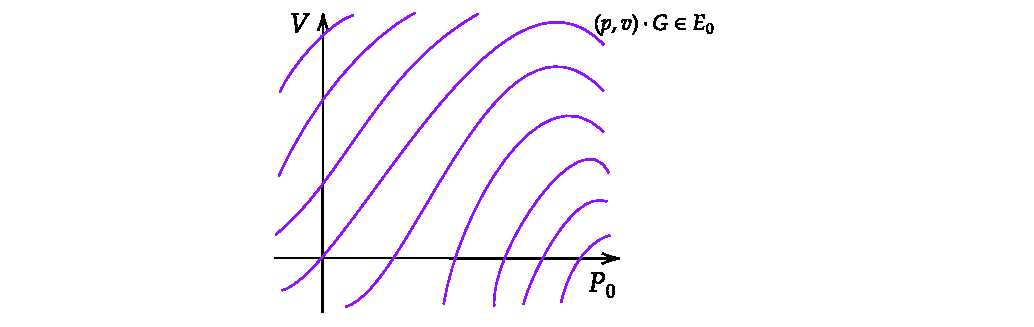
\includegraphics[trim={47mm 4mm 51mm 0},clip,width=\textwidth]{figs/associated_fiber_integral.pdf}
		\end{minipage} 
		\begin{minipage}[c]{0.48\textwidth}
	        \caption{Elements of the fiber $E_0$ viewed as orbits of $P_0\times
			V$. The diagram reflects $G$ being a free action on  $P_0$, but not
			necessarily on $V$}
	        \label{fig:associated_fiber_integral}
		\end{minipage} 
	\end{figure}
	The tangent space at $(p,v)\in P_0\times V$ 
	is $V_pP \oplus V$. But the connection on $P\times V$ is the pullback 
	$p_1^*\omega$, which is constant in the $V$ direction, and the curvature
	form vanishes on  $V_pP\oplus V$ since it is a horizontal form. 
	If $\alpha_1,\ldots,\alpha_d$ is a dual basis for
	$\g^*$, the element $p_2^*U$ is a sum of terms of the form 
	$\beta_I \alpha_I$, where  $\beta_I \in \Omega(P\times V)$ are invariant
	forms. 
	After we replace the $\alpha_i$ by the curvature forms  $\Omega_i$, as a
	form on $P_0\times V$ we are only left with the term $\beta_0$. 
	Then taking the horizontal component amounts to only evaluating tangent
	vectors in $V$ at each point $(p,v)\in P_0\times V$. 
	Subsequently, the fiber integral is the same as the integral of 
	$\beta_0$ over $V$, which equals 1 because $\int_V U = 1$.  
	\begin{comment} % first attempt
	This is defined on $\Omega(P\times_G V)\simeq \Omega(E)$ in exactly the same
	way, since coordinate functions on $E$ can be pulled back via the canonical
	isomorphism to coordinate functions on $P\times_G V$. 
	Recall that a local trivialisation 
	$\phi_\alpha : E|_{U_\alpha} \to U_\alpha \times
	\mathbb{R}^n$ gives coordinate functions $[t_1\cdots t_n] = p_2\phi_\alpha
	\in \mathbb{R}^n$ where $p_2$ is the projection on to $\mathbb{R}^n$.  
	This can be identified with coordinate functions on the associated bundle
	$[x_1\cdots]$
	\end{comment}
\end{proof}

The above theorem is proved in chapter 10 of \cite{guillemin} in the more
general context of a $K$-manifold $E=P\times_\rho V$, and a principal
$G$-bundle  $P\times V \to P\times_\rho V$, with associated Cartan map
$\Car_\omega : \Omega_{G\times K}(P\times V)\to\Omega_K(E)$. The Thom form is
obtained from the map $\Car_{\omega}(p_2^*U)$ where $U\in\Omega_{G\times K}(V)$.

% Guillemin 7.2
We shall now construct the Mathai-Quillen universal Thom form.
Let $V$ be a real vector space with standard inner product, and $\rho : G \to
\SO(V)$ be a rep of the Lie group $G$, with induced rep $\rho_* :
\mathfrak{g}\to \so(V)$.
We will apply the Berezin integral to a form in $S(\mathfrak{g}^*)\otimes 
\Omega(V) \otimes \bigwedge V$. 
Fix an oriented orthonormal basis $\{e_1,\ldots,e_n\}$ for
$V$, which allows us to define the Berezin integral, with corresponding
coordinate functions $x_1,\ldots,x_n$.   
Let  $\{X_1,\ldots,X_m\}$ be a basis of $\mathfrak{so}(V)$, with corresponding
dual basis $\{u_1,\ldots,u_m\}$ where $m= \frac{1}{2}n(n-1)$. Recall that we 
can identify $\mathfrak{so}(V)$ with 
$\bigwedge^2 V$ via equation (\ref{eq:so_wedge}), restated here 
\[
	X_a \in\mathfrak{so}(V) \mapsto \sum_{i<j}\gen{X_a e_i,e_j} e_i\wedge e_j
	= \frac{1}{2}\sum_{i} e_i\wedge X_a e_i
\] 
Denote $dx := \sum_i dx_i \otimes e_i \in \Omega^1(V)\otimes V$. Define the element 
\begin{equation} % 7.16 guillemin % cordes eq 11.13 % naber 3.18
	\label{eq:universal_thom_exponent}
	\sigma := -\frac{1}{2}\abs{x}^2 - idx 
	- \sum_a u_a\rho_* \otimes X_a 
	\quad \in S(\g^*) \otimes \Omega(V) \otimes \bigwedge V
\end{equation}
which is analogous to $\omega_1$ as defined in Prop \ref{prop:closed_prop}.
Note that $u_a \rho_* \in \mathfrak{g}^*$.
In components, if $M^a = [\gen{ X_ae_i,e_j}]_{ji}$, we can write the same
element as 
\begin{equation} \label{eq:universal_thom_exponent2}
\sigma = -\frac{1}{2}\abs{x}^2 - i\sum_i dx_i\otimes e_i 
	-\frac{1}{2} \sum_{i,j} (\rho_*)_{ji}e_i\wedge e_j
\end{equation}
since $u_aX_a$ is the identity on  $\so(V)$, and $(\rho_*)_{ji} \in \mathfrak{g}^*$.
Consider its Berezin integral
\begin{equation} \label{eq:universal_thom}
	U := \epsilon(n)(2\pi)^{-n /2}\int^B \exp\paren{\sigma}  
	\quad\in S(\g^*)\otimes \Omega(V)
\end{equation}
where $\epsilon(n)=1$ if $n$ is even and otherwise $\epsilon(n)=i$.

\begin{thm} \label{thm:uinversal_Thom}
	The element $U \in S(\mathfrak{g}^*) \otimes \Omega(V)$ defined above  
	is a universal Thom form.
\end{thm}
\begin{proof} % Guillemin p86-87
We need to show that it is invariant and
equivariantly closed in the Cartan model, and integration along the
fiber gives 1. 


(1) Closed. 
We can consider the Cartan
differential $\delta_C = d - \sum u_k\iota_k$ as an operator on 
$S(\so(V)^*)\otimes\Omega(V)\otimes\bigwedge V$ by acting trivially on
the last factor, so that it commutes with the Berezin integral. 
It suffices to show $U$ is closed as a form on  $S(\so(V)^*)\otimes \Omega(V)$,
because the map  $\rho^* : S(\so(V)^*)\to S(\g^*)$ given by  $u_i\mapsto
u_i\circ \rho_*$ commutes with the Cartan differential. This can be seen most
easily by viewing the elements as polynomials as in Theorem
\ref{thm:cartan_diff}, which shows that  $(\delta_C \rho_* \alpha)(X) 
= (\rho_*\delta_C \alpha)(\rho(X)) = (d-\iota_{\rho(X)})\alpha(\rho(X))$, noting
that $\iota_X$ and  $\iota_{\rho(X)}$ act the same way on $\Omega(V)$.

For the first term, only $d$ acts to give $\delta_C \abs{x}^2 = 2x_i dx_i$.
On the second term, $d^2=0$ and we need to evaluate $u_a\iota_a dx_i$. 
Since $x_i$ projects to the $i$th component of a vector in $V$, and the action
of $e^{tX_k}$ is matrix multiplication, for $v\in V$ in the tangent space
\begin{align} \label{eq:interior_dx}
	\iota_a dx_i(v)
	= d x_i \paren{\odv{}{t}_{t=0} e^{-tX_a} v} 
	= -x_i \paren{X_a v} 
\end{align}
Hence, $u_a\iota_a dx_i = -u_a\otimes x_i \circ X_a$. The third term is a
multiple of $u_i$ and constant on $\Omega(V)$,
hence maps to zero by  $\delta_C$. Thus, 
\begin{align}
	(d-u_a\iota_a) \sigma 
&= -x_i dx_i - u_a \otimes i x_iX_a \otimes e_i \nonumber \\
&= -x_i dx_i - u_a \otimes i x_j \otimes X_a e_j 
\end{align}
which is justified by $x_j$ being the coordinate functions of $e_j$:
\begin{equation} \label{eq:move_operator_tensor}
x_i X_a \otimes e_i 
= \gen{X_ae_j,e_i}x_j \otimes e_i 
= x_j \otimes \gen{X_ae_j,e_i}e_i 
= x_j \otimes X_a e_j 
\end{equation}
The key observation is that $\delta_C$ acts by lowering the degree of the
$\bigwedge V$ part. More precisely, consider the action of the Berezin
derivative/integral
\begin{align*}
\pdv{}{e_k} \paren{-\sum_{i<j} u_a\otimes e_i\wedge M^a_{ji}e_j}
&= -\sum_{i>k} u_a\otimes M^a_{ik}e_i + 
 \sum_{i<k} u_a\otimes M^a_{ki}e_i \\
&= -\sum_{i} u_a\otimes M^a_{ik}e_i  
= -u_a\otimes X_a e_k  
\end{align*}
since $M^a_{ij}=-M^a_{ji}$. Applying $\pdv{}{e_k}$ to the other term,
\[
\pdv{}{e_k} (-idx_i \otimes e_i) = idx_k
\] 
because $e_i$ anti-commutes with  $dx_i$. We have shown that
\begin{equation}
\delta_C \sigma = \paren{\sum_{k} ix_k \pdv{}{e_k}}\sigma
\end{equation}
It follows that this also holds for $\exp (\sigma)$, because  $\delta_C$ is an
anti-derivation. Therefore, 
\[
\delta_C \int^B \exp(\sigma) 
= \int^B \delta_C \exp(\sigma)
= \int^B ix_k \pdv{}{e_k} \exp(\sigma) = 0
\] 
as the Berezin derivative kills any top degree terms in $\bigwedge V$.

(2) Integral along the fiber. We need to extract the coefficient of $dx_1\wedge
\ldots\wedge dx_n$. Therefore, the last term in $\sigma$ does not contribute,
and 
 \[
	 \int_V U = \epsilon(n)(2\pi)^{-n /2}\int_V e^{-\abs{x}^2} \int^B \exp(-idx_k \otimes e_k) 
\] 
But we know $\int^Be^{-idx_k\otimes e_k}$ evaluates to 
$(-i)^n(-1)^{n(n-1)/2} dx_1\wedge \ldots\wedge dx_n$ by Lemma
\ref{lem:gaussian_integral}. Hence, the integral of $U$ along the fiber $V$ is 1.

(3) Invariant. % proved in p27 Constantinecu PhD
It suffices to show the terms in $\sigma$ are invariant, because
the Lie derivative is a derivation. We can extend the action of $G$ to the
graded algebra $S(\g^*)\otimes \Omega(V)\otimes \bigwedge V$,
acting on the $\bigwedge V$ component by multiplication by $\rho(g)^{-1}$. 
Note that the Berezin integral is
invariant under the action on $\bigwedge V$. This gives an associated Lie derivative,
corresponding to multiplication by $\rho_*(X)$ for  $X\in\mathfrak{g}$.

It is clear that $\abs{x}^2$ is invariant, because $\rho(g)$ has determinant 1.
Next, we show $dx_i\otimes e_i$ is invariant by applying $\mathcal{L}_X$,
\[
\mathcal{L}_X (dx_i\otimes e_i) = \iota_X(dx_i) \otimes e_i + dx_i \otimes
\rho_*(X)e_i = 0
\] 
by equations (\ref{eq:interior_dx}) and (\ref{eq:move_operator_tensor}).
Finally, to apply $\mathcal{L}_X$, recall that the action on $S(\g^*)$ 
is the coadjoint representation $\mathcal{L}_X \alpha(Y) = -\alpha ([X,Y])$. 
The action on $V$ is  $\mathcal{L}_X v = \rho_*(X)v$.
We can denote the third term in $\sigma$
as $\frac{1}{2}e_i\wedge (\rho_*)_{ji} e_j \in \g^*\otimes \bigwedge^2V$,
since $u_aX_a$ is just the identity.
For $X,Y\in\g$, with  $\rho_*(X)=A,\rho_*(Y)=B$,
\begin{align*}
	&\quad\;(\mathcal{L}_X(e_i \wedge (\rho_*)_{ji} e_j))(Y) \\
	&= (A e_i \wedge \rho_* e_i)(Y)
	- e_i \wedge \rho_*([X,Y]) e_i
	+ (e_i \wedge \rho_* A e_i)(Y) \\
	&= Ae_i \wedge B e_i
	- e_i \wedge (AB-BA) e_i
	+ e_i \wedge A Be_i \tag{$\star$} \\
	&= -e_i \wedge BA e_i
	- e_i \wedge (AB-BA) e_i
	+ e_i \wedge AB e_i = 0\tag{$\star\star$}
\end{align*}
where we begin by using the derivation property of $\mathcal{L}_X$, and explain
the next two lines below.

Proof of ($\star$): This step initially looks wrong, but recall that the term is
to be interpreted as 
\[
\sum_{i,j}e_i\wedge (\rho_*(Y))_{ji} (Ae_j)
=\sum_{i,j}e_i\wedge \sum_kB_{ji} A_{kj}e_k
=\sum_{i}e_i\wedge \sum_{k,j}A_{kj}B_{ji} e_k
=\sum_{i}e_i\wedge AB e_i
\] 
Proof of ($\star\star$): This is just an application of the more general property
\[
Ae_i \wedge Be_i
= A_{ji}e_j \wedge B_{ki}e_k
= e_j \wedge B_{ki}A^\intercal_{ij}e_k
= e_j \wedge BA^\intercal e_j 
\] 
Finally, $U$ is invariant because $\mathcal{L}_X$ commutes with the Berezin
integral.
\end{proof}

The proof of (1) closure is due to \citet{guillemin} and part of (3) invariance
is a corrected version of the proof in \citet[p.27]{constantinescu}. In
particular, the steps $(\star)$ and  $(\star\star)$ are corrected, as well as
the action of $\mathcal{L}_X$ on $\mathfrak{g}^*$. 

\begin{remark}
	The minus sign in $e^{-tX_a}$ in the fundamental vector field over $V$ in
	equation (\ref{eq:interior_dx}) arises due to the fact that the
	$\SO(V)$-action on $V$ is a right action. In general, this is so that the
	map $\g \to \Gamma(TM)$ is a Lie algebra homomorphism. 
\end{remark}	
 
% TODO prove equivalence to usual form
To relate our formula to other versions in literature, let $\chi =
(e_1,\ldots,e_n)$ be the Grassman variables for $V$. 
In more compact notation, the third term of $\sigma$ can be written  
as $\frac{1}{2} e_i \wedge (\rho_*)_{ij} e_j = \frac{1}{2} \chi^\intercal
(\rho_*) \chi$. Then the Mathai-Quillen Thom form 
$U\in S(\mathfrak{g}^*)\otimes \Omega(V)$ can be alternatively written as 
\begin{equation} \label{eq:universal_thom_form} % AJ 2.1
	U = \epsilon(n)(2\pi)^{-n /2}e^{-\abs{x}^2 /2} 
	\int^B \exp \paren{\frac{1}{2}\chi^{\intercal}(\rho_*)\chi -
idx^{\intercal}\chi} \odif{\chi} 
\end{equation}
If $\rho_*(X)\in\so(V)$ is always invertible, we can apply
Proposition \ref{prop:berezin_formula}, to get
\[
U = \epsilon(n)(2\pi)^{-n/2} \Pf(\rho_*) \exp(-\abs{x}^2 /2-dx^{\intercal} (\rho_*)^{-1}dx)
\] 
We can also obtain a universal Thom form in the Weil model, by 
applying the Weil-Cartan isomorphism $(S(\mathfrak{g}^*)\otimes \Omega(V))^G
\xrightarrow{\simeq}(W(\mathfrak{g})\otimes \Omega(V))_{bas}$. 

\begin{comment} % Mathai-Quillen forms in Weil model 
\[% cordes eq11.12
		U = (2\pi)^{-m} \Pf(\phi) \exp(-\abs{x}^2-\gen{\nabla x,\phi^{-1}\nabla x})
\] 
\[%MQformula weil eq 6.2 (extended from 1.8)
	U = (2\pi)^{-m}\Pf(\Omega) \exp(-x^2-(dx+\theta x)^\intercal \Omega^{-1}
	(dx+\theta x))
\]
\end{comment}


\vspace{5mm}
\hrule 
\vspace{5mm}

\textbf{Bibliographical notes}
{\small
\begin{itemize}
	\item A more comprehensive treatment of the Thom isomorphism can be found in
		\citet{bott_tu}.  
	\item The Mathai-Quillen formula described in section
		\ref{section:mq_formula} is based on section 
		section 1.6 of \cite{bgv}.
	\item The book by \citet{guillemin} gives an exposition of the
	Mathai-Quillen formula in the equivariant case 
\end{itemize}
}
